\documentclass{beamer}

\usepackage{gensymb}
\input{entete_beamer_pdflatex}
\usepackage{listings}
\lstset{language=Python, tabsize=2, breaklines=true, showstringspaces=false}

\useoutertheme{infolines}
\setbeamersize{text margin left=1cm,text margin right=1cm}

\title{Rapport de projet de SI}
\subtitle{Tropodrone}
\author{Gueydan Noé, Manceau Thibaut, Gros Alexis, Porteries Tristan}

\begin{document}

\begin{frame}
  \titlepage
\end{frame}

\begin{frame}
    \frametitle{Sommaire}
    \begin{multicols}{2}
      {
		\setcounter{tocdepth}{1}
        \tableofcontents
      }
    \end{multicols}
\end{frame}

\section{Courte présentation}

\subsection{But du projet}

\begin{frame}
 Créer une structure composée de ballons contenant un gaz plus léger que l’air qui soutient une partie ou la totalité du poids d'un drone.
\end{frame}


\subsection{Objectifs}

\begin{frame}
 Augmenter l’autonomie, la sécurité et les possibilités d’un drone de petite taille
\end{frame}


\subsection{Contraintes imposées au projet}
\begin{frame}
  \begin{itemize}
    \item Être simple d’utilisation, garder la manœuvrabilité du drone au possible pour le drone, voler le plus longtemps possible.
    \item Consommer le moins d’énergie possible, ne pas présenter de danger pour le public et économiser le gaz et les matériaux de fabrication.
    \item Le modèle du drone imposé
    \item Rayon d’action de minimum 15 mètres
    \item Ballon de type dirigeable
  \end{itemize}
\end{frame}

\subsection{Contraintes légales supplémentaires}
\begin{frame}
  \begin{itemize}
    \item 1: Le drone \\
	    Catégorie A : limitations non contraignantes
    \item 2: Le ballon \\
	    Catégorie « Léger » \\
	    La ficelle supportant la charge doit casser au dessus de 23 kg
 \end{itemize}
\end{frame}


\section{Structure}

\subsection{Gyroscope et axes}

\begin{frame}
  
\end{frame}

\subsection{Attaches et modélisation}

\section{Ballon}

\subsection{Contenance}

\subsection{Forme}

\begin{frame}
  Les ballon sont formés d'un parallèlépipède avec deux pyramides d'angle $60\degree$. \\
  \begin{center}
    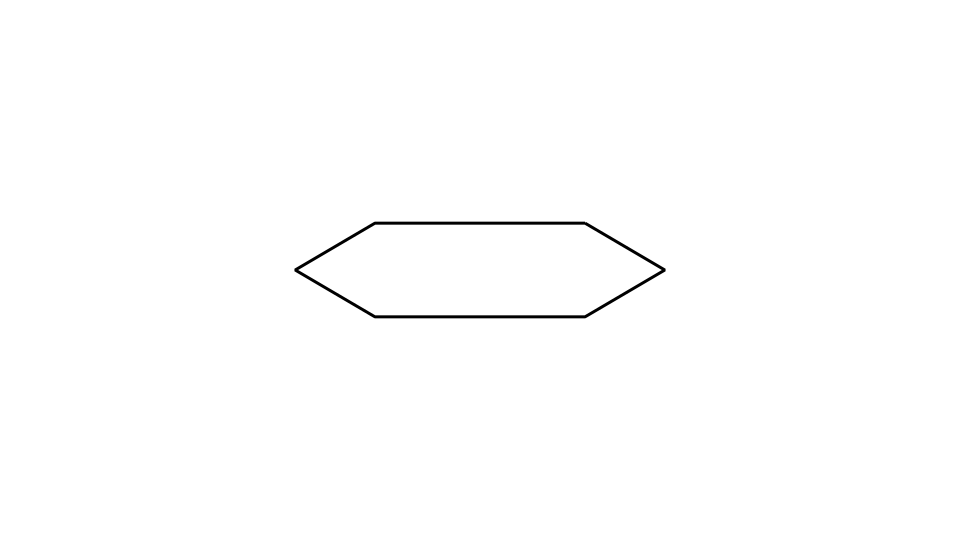
\includegraphics[width=10cm]{../Images/ballon.png}
  \end{center}
\end{frame}

\begin{frame}{Calcul des dimensions}
  Volume ballon~:
  \begin{center}
    \medbreak
    $b^3 \sin \frac{\pi}{3} \times \frac{1}{3} + b^2$
  \end{center}
  Polynome du troisième degrée, résolution par bissection ou dichotomie.
\end{frame}

\begin{frame}[fragile]{Résolution par bissection}
  \begin{lstlisting}[frame=single]
etape = 1
largeur = 1
vol = volume(largeur)
cible = 0.25
epsilon = 1e-4
while abs(vol - cible) > epsilon:
	if vol < cible:
		largeur += etape
	else:
		largeur -= etape
	etape /= 2
	vol = volume(largeur)

print("volume = %f, diametre = %f" % (vol, largeur))
  \end{lstlisting}
\end{frame}

\subsection{Enveloppe}

\begin{frame}
  \begin{multicols}{2}
    \begin{itemize}
      \item Latex~:
      \begin{itemize}
        \item Facile à trouver dans le commerce,
        \item Seulement en forme sphèrique,
        \item Peu étanche~;
      \end{itemize}
      \item Chloroprène~:
      \begin{itemize}
        \item Introuvable dans le commerce~;
      \end{itemize}
      \item Butyle~:
      \begin{itemize}
        \item Introuvable dans le commerce~;
      \end{itemize}
    \end{itemize}
    \newpage
    \begin{itemize}
      \item Mylar~:
      \begin{itemize}
        \item Facile à trouver dans le commerce~;
        \item Resistant à la traction~;
        \item Peu être assembler~;
        \item Peu élastique~;
        \item Fragile au cisaillement.
      \end{itemize}
    \end{itemize}
  \end{multicols}
\end{frame}

\subsection{Collage}

\begin{frame}
  \begin{itemize}
    \item Néoprène(Polychloroprène)
    \begin{itemize}
      \item Etanche
      \item Elastique
      \item Adhèrent
      \item Difficile à appliquer
    \end{itemize}
    \item 406 et 770
    \begin{itemize}
      \item Peu adhèrent
      \item Rigide
      \item Difficile à appliquer
    \end{itemize}
  \end{itemize}
\end{frame}

\subsection{Gonflage}

\section{Calculs d'élévation}

\subsection{Poussé d'archimède}
\subsection{Dilatation des gaz}

\begin{frame}{Loi de Charles}
  \begin{center}
    $\frac{V_1}{T_1} = \frac{V_2}{T_2} = f(P, n)$
    \bigbreak
    $V_3 = f(P, n) \times T_3$
  \end{center}
  \bigbreak
  $V_q$~: volume du gaz à la température $T_q$. $P$~: pression du gaz. $n$~: quantité de matière. $f(P, n)$~: rapport constant entre volume et température.
\end{frame}

\begin{frame}{Application à l'hélium}
  Volume molaire de l'hélium~: $22.414\times 10^{-3} m^3.mol^{-1}$ à $273.25K$.
  \medbreak
  \begin{center}
    $f(P, n) = \frac{22.414\times 10^{-3}}{273.25} = 8.2\times 10^{-5} m^3.mol^{-1}.K^{-1}$
    \bigbreak
  \end{center}
  Pour $T_{200} = 200 \degree C = 473.25 K$~:
  \begin{center}
    \medbreak
    $V_{T_{200}} = 8.2\times 10^{-5} * 473.25 = 38.811 \times 10^{-3}$
  \end{center}
  Augmentation du volume de $1.59$.
\end{frame}

\begin{frame}{Résultat de la poussé d'archimède}
  \begin{center}
    $F_{T_0} = P_{air} - P_{helium} = 10.90 N$
    \bigbreak
    $F_{T_{200}} = P_{air} - \frac{P_{helium}}{1.59} = 11.57 N$ \\
  \end{center}
  Les resultats sont négligables. $F < P_{air}$
\end{frame}

\section{Drone}

\subsection{Modèle}
\subsection{Capacité et poids}

\section{Aérodynamisme}

\subsection{Équation de traînée}
\begin{frame}
 But : que le drone soit le moins sensible à l'air possible \\
 Force de traînée matérialisée par l'équation \\
 \begin{center}
  $\frac12 \rho S Cx V^2$
 \end{center}
\end{frame}

\subsection{Calcul de Cx pour la forme retenue 1/2}
\begin{frame}
 Forme la plus proche : sphère \\
 Dépend du type d'écoulement : le nombre de reynolds \\
 \begin{center}
  \begin{tabular}{lll}
   $Re < 1$ & $Cx = $ & $\frac{24}{Re}$ \\
   $1 < Re < 10^3$ & $Cx = $ & $\frac{18.5}{Re^0.6}$ \\
   $10^3 < Re < 5.10^5$ & $Cx = $ & $0.44$
  \end{tabular}
 \end{center}
\end{frame}

\subsection{Calcul de Cx pour la forme retenue 2/2}
\begin{frame}
 \begin{center}
  $Re = \frac{VL}{\nu}$
 \end{center}
 Avec : \\
 V Vitesse du fluide en m/s \\
 L Diamètre en m \\
 $\nu$ Viscosité cinématique en $m^2/s$ \\
 ($\nu = 15.6*10^6$ pour l'air)
\end{frame}

\end{document}
